\documentclass[11pt,a4paper]{article}

\usepackage[a4paper,margin=1in]{geometry}
\usepackage{graphicx}
\usepackage{booktabs}
\usepackage{float}
\usepackage{hyperref}
\usepackage{xcolor}
\usepackage{listings}
\usepackage{enumitem}
\usepackage{fancyhdr}

\hypersetup{colorlinks=true,linkcolor=blue,urlcolor=blue}

\pagestyle{fancy}
\setlength{\headheight}{14pt}
\fancyhf{}
\lhead{Computer Networks Laboratory}
\rhead{Assignment 5}
\cfoot{\thepage}

\lstdefinestyle{cstyle}{
  language=C,
  basicstyle=\ttfamily\small,
  numbers=left,
  numberstyle=\tiny,
  frame=single,
  breaklines=true,
  showstringspaces=false,
  keywordstyle=\color{blue},
  commentstyle=\color{gray},
  stringstyle=\color{purple}
}
\lstset{style=cstyle}

\setlength{\parskip}{0.5em}
\setlength{\parindent}{0pt}

\begin{document}

\begin{center}
{\LARGE \textbf{Assignment 5: Simulation of Domain Name Resolution Using UDP Socket Programming}}\\[4mm]
Simiyon Vinscent Samuel L\\
Register Number: 3122247001062\\
Submission Date: August 18, 2026\\
GitHub Repository: \url{https://github.com/blackscythe123/PCN-assign}
\end{center}

\vspace{2mm}
\hrule
\vspace{4mm}

\section*{Aim}
To simulate a DNS server and client over UDP in C -- the server holds a small
hostname-to-IP table and answers lookups, the client caches recent resolutions
locally, validates input before sending anything, and times out cleanly if the
server never replies. The bigger point of the exercise is to actually see, not
just claim, that the client-side cache avoids a real network round-trip, and
that a UDP client left alone with a dead server will hang forever unless you
code a timeout yourself.

\section*{DNS Server -- dns\_server.c}
\texttt{dns\_server.c} listens on UDP port 6062 with a plain
\texttt{recvfrom()}/\texttt{sendto()} loop -- no \texttt{listen()}/\texttt{accept()}
since UDP has no connections. The ``DNS table'' is just a fixed array of
10 \texttt{struct DnsEntry\{hostname, ip\}} pairs (fictional domains like
\texttt{www.example.com}, \texttt{mail.college.edu}, \texttt{portal.ssn.edu.in}),
searched linearly. That is genuinely all a lab-scale DNS table needs -- no hash
map, no persistence.

\begin{lstlisting}[caption={dns\_server.c -- table lookup and the FOUND / NXDOMAIN reply}]
char *lookup_hostname(char *hostname) {
    int i;
    for (i = 0; i < entry_count; i++) {
        if (strcmp(dns_table[i].hostname, hostname) == 0) {
            return dns_table[i].ip;
        }
    }
    return NULL;
}

char *ip = lookup_hostname(buf);
if (ip != NULL) {
    snprintf(response, sizeof(response), "FOUND %s", ip);
} else {
    snprintf(response, sizeof(response), "NXDOMAIN");
}
\end{lstlisting}

\section*{DNS Client -- dns\_client.c}
\texttt{dns\_client.c} reads hostnames one per line from stdin and, for each
one, runs through: format validation, then a cache check, and only on a cache
miss does it actually touch the network.

\begin{lstlisting}[caption={dns\_client.c -- cache check BEFORE sending anything over UDP}]
char *cache_lookup(char *hostname) {
    int i;
    for (i = 0; i < cache_count; i++) {
        if (strcmp(cache[i].hostname, hostname) == 0) {
            return cache[i].ip;
        }
    }
    return NULL;
}
...
char *cached_ip = cache_lookup(line);
if (cached_ip != NULL) {
    printf("  CACHE HIT: %s -> %s (no UDP query sent)\n", line, cached_ip);
    continue;   /* skips sendto()/recvfrom() entirely */
}
printf("  CACHE MISS: querying DNS server...\n");
\end{lstlisting}

\begin{lstlisting}[caption={dns\_client.c -- basic hostname format validation, run before any socket call}]
int is_valid_hostname(char *hostname) {
    int len = strlen(hostname);
    int i, has_dot = 0;
    if (len == 0 || len > 63) return 0;
    for (i = 0; i < len; i++) {
        char c = hostname[i];
        if (isalnum((unsigned char)c) || c == '.' || c == '-') {
            if (c == '.') has_dot = 1;
        } else {
            return 0;  /* invalid character */
        }
    }
    if (!has_dot) return 0;  /* no dot -- not a plausible hostname */
    return 1;
}
\end{lstlisting}

\begin{lstlisting}[caption={dns\_client.c -- SO\_RCVTIMEO so a dead server can never hang the client}]
tv.tv_sec = TIMEOUT_SEC;   /* 2 seconds */
tv.tv_usec = 0;
setsockopt(sockfd, SOL_SOCKET, SO_RCVTIMEO, &tv, sizeof(tv));
...
int n = recvfrom(sockfd, response, BUF_SIZE - 1, 0,
                  (struct sockaddr *)&from_addr, &from_len);
if (n < 0) {
    /* SO_RCVTIMEO expired with no reply -- this is the timeout path */
    printf("  TIMEOUT: no response from DNS server within %d seconds.\n", TIMEOUT_SEC);
    continue;
}
\end{lstlisting}

\section*{Testing}
All five required cases were run headlessly through WSL Ubuntu and logged
under \texttt{as5/logs/}.

\begin{itemize}
\item \textbf{First lookup (cache miss):} queried \texttt{mail.college.edu} --
client printed \texttt{CACHE MISS: querying DNS server...} then
\texttt{RESOLVED: mail.college.edu -> 10.20.30.40}. The server log shows one
matching \texttt{Query received ... "mail.college.edu"} line. (\texttt{01\_first\_lookup.txt})
\item \textbf{Same lookup again (cache hit):} the very next query for the same
hostname, in the same client session, printed
\texttt{CACHE HIT: mail.college.edu -> 10.20.30.40 (no UDP query sent)} with no
new server round-trip. Checked the server's own log for that whole session --
it shows \textbf{exactly one} query for \texttt{mail.college.edu}, not two, which
is the real proof the cache was actually used and not just decorative.
(\texttt{02\_cache\_hit.txt}, cross-checked against \texttt{server\_session\_tests1to4.txt})
\item \textbf{Non-existent domain:} queried \texttt{nosuchdomain.xyz}, not in
the table. Server logged \texttt{NXDOMAIN (not in table)} and the client printed
\texttt{NXDOMAIN: "nosuchdomain.xyz" does not exist in the DNS table.}
(\texttt{03\_nxdomain.txt})
\item \textbf{Invalid format:} tried \texttt{bad\_host!!name} (bad characters)
and \texttt{localhost} (no dot). Both were rejected client-side with
\texttt{ERROR: invalid hostname format, not sending to server.} before any
socket call -- confirmed neither line shows up anywhere in the server log.
(\texttt{04\_invalid\_format.txt})
\item \textbf{Genuine timeout:} killed the DNS server first (checked with
\texttt{pgrep dns\_server} returning empty), then ran the client against the
now-dead port 6062. It printed \texttt{TIMEOUT: no response from DNS server
within 2 seconds.} and returned normally instead of hanging. Timed the whole
run with \texttt{/usr/bin/time}: \texttt{elapsed\_wall\_clock\_seconds=2.10},
which lines up with the \texttt{TIMEOUT\_SEC = 2} set via
\texttt{SO\_RCVTIMEO} in the code -- so this is a real, measured timeout, not
just a printed claim. (\texttt{05\_timeout.txt})
\end{itemize}

\begin{figure}[H]
\centering
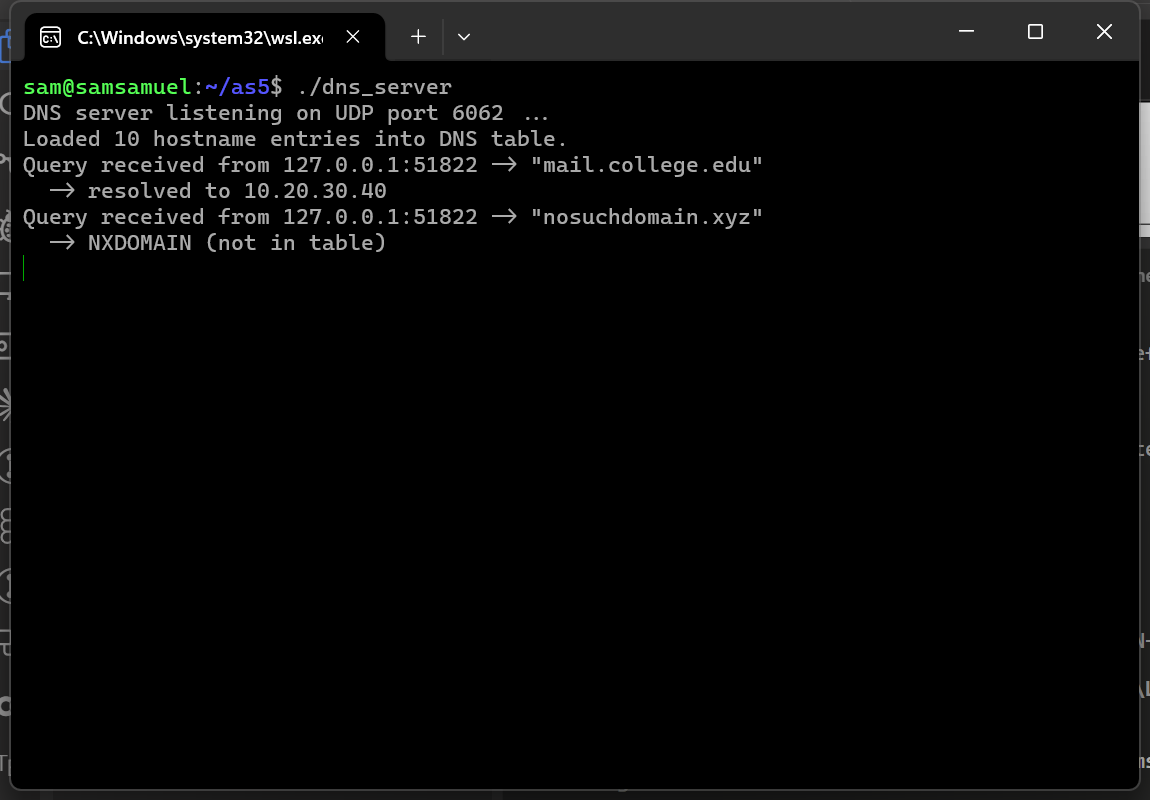
\includegraphics[width=0.85\linewidth]{ss/01_dns_server.png}
\caption{DNS server terminal, running, showing incoming query log lines for
successful lookups and an NXDOMAIN case.}
\end{figure}

\begin{figure}[H]
\centering
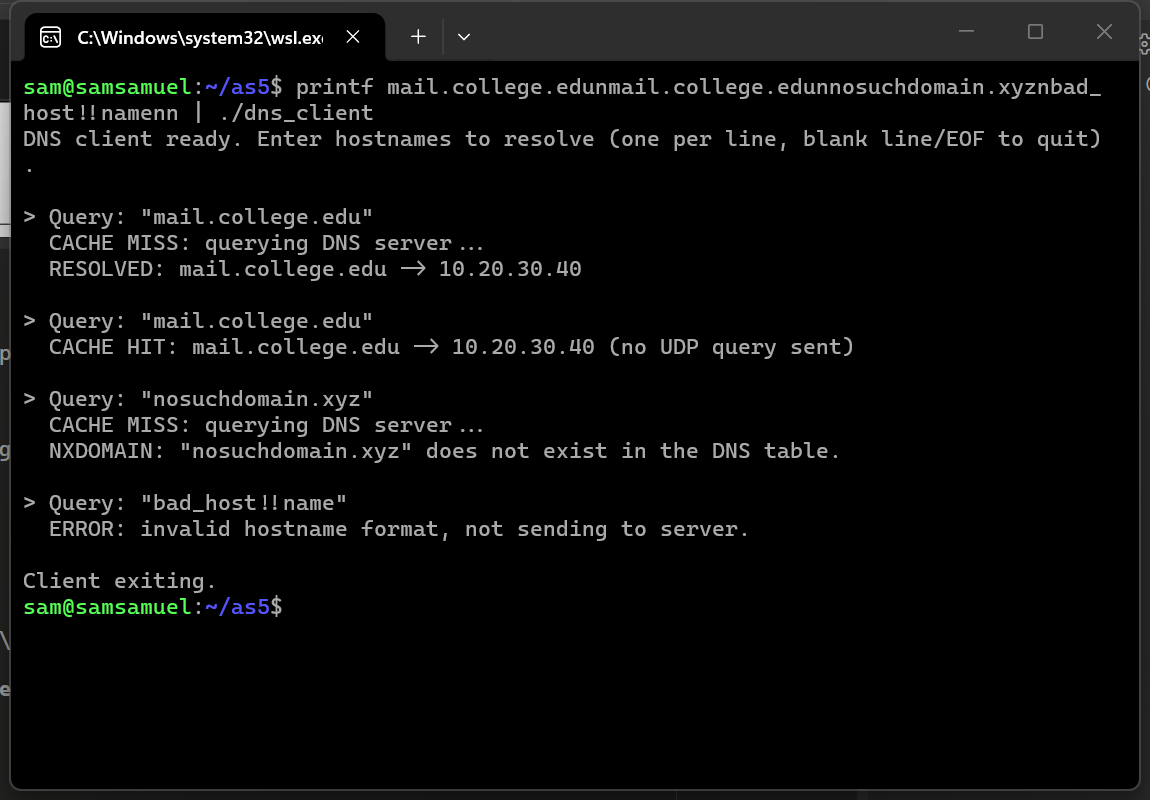
\includegraphics[width=0.85\linewidth]{ss/02_dns_client_lookups.png}
\caption{DNS client terminal, one run, in sequence: first lookup (cache miss,
hits server), the same lookup again (cache hit, no server round-trip), the
NXDOMAIN case, and the invalid-format case.}
\end{figure}

\begin{figure}[H]
\centering
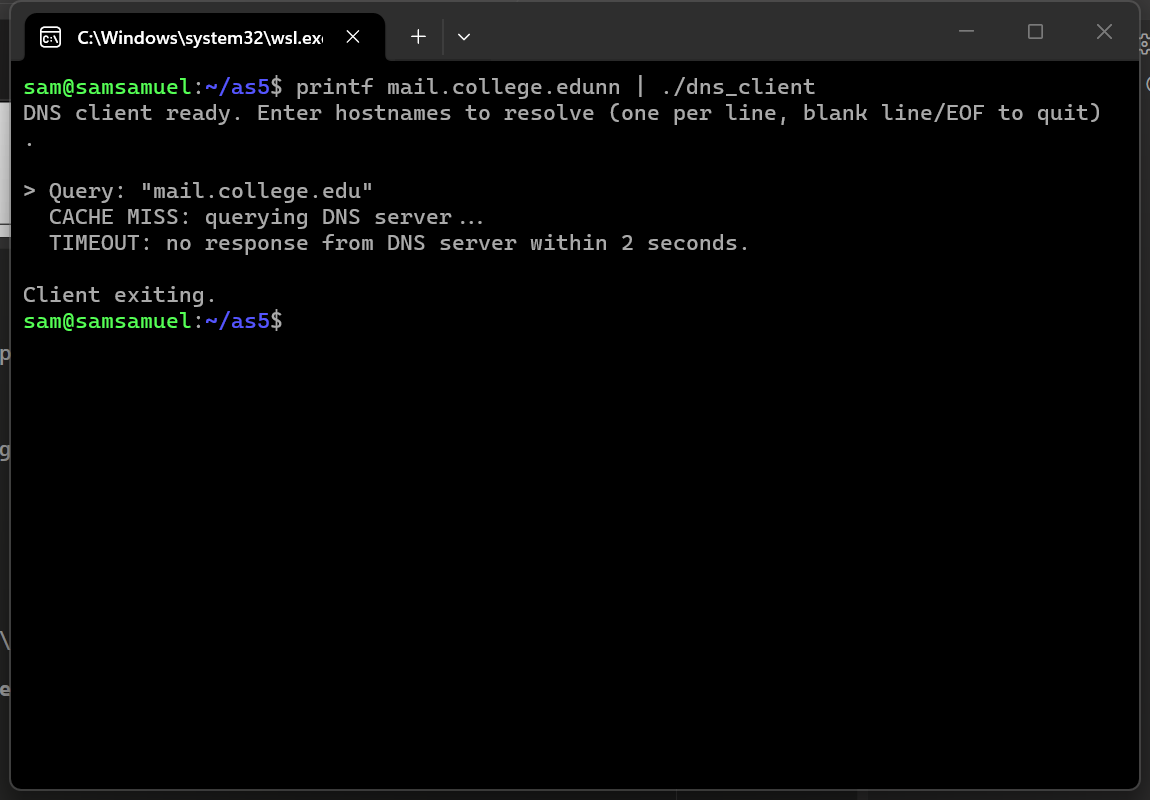
\includegraphics[width=0.85\linewidth]{ss/03_dns_client_timeout.png}
\caption{Separate client run against a dead server showing the genuine
SO\_RCVTIMEO timeout firing after roughly two seconds.}
\end{figure}

\section*{Is UDP Actually a Good Fit for DNS?}
\begin{itemize}
\item \textbf{Overhead:} No handshake, no connection state on either side --
each query is a single small datagram out and a single small datagram back.
For something as short and frequent as a hostname lookup this is a lot cheaper
than paying for a TCP three-way handshake every time.
\item \textbf{Latency:} Because there's no setup step, a successful lookup is
about as fast as a single round-trip can be -- exactly what a client blocking
on a page load actually wants.
\item \textbf{Reliability:} This is the catch, and this lab makes it concrete:
UDP itself gives zero delivery guarantee. \texttt{sendto()} ``succeeds'' even
if nothing is listening, and without the \texttt{SO\_RCVTIMEO} we added by
hand, \texttt{dns\_client.c} would just block on \texttt{recvfrom()} forever if
a packet (or the server) vanished. Real DNS resolvers handle this the same
way -- application-level timeout and retry -- rather than falling back to TCP
for every query. So UDP is a good fit \emph{only because} the application is
willing to take on that responsibility itself, which is exactly what the
caching + timeout logic in this client is doing.
\end{itemize}

\section*{Learning Outcome}
\begin{itemize}
\item Building the client-side cache was easy to write but easy to get wrong
in a way that looks right -- the real test wasn't the client printing
``CACHE HIT'', it was going back to the server's own log and seeing only one
entry for the repeated hostname.
\item \texttt{SO\_RCVTIMEO} genuinely changes program behaviour -- without it
the client hung indefinitely against a dead port when I first tried it; with
it, killing the server mid-test and re-querying reliably came back in about
two seconds instead of never.
\item Writing \texttt{is\_valid\_hostname()} was a reminder that ``validate
the input'' is a real design decision, not a formality -- e.g. I had to decide
that a blank line means ``quit the client'' rather than ``query an empty
hostname'', which meant the empty-string case had to be tested through the
function's own logic rather than as a live client query.
\end{itemize}

\end{document}
